\documentclass[conference]{IEEEtran}
\IEEEoverridecommandlockouts

\usepackage{cite}
\usepackage{amsmath,amssymb,amsfonts}
\usepackage{graphicx}
\usepackage{booktabs}
\usepackage{array}
\usepackage{url}
\usepackage{xcolor}
\usepackage{tikz}
\usetikzlibrary{arrows.meta,positioning}

% Figures are read straight from the pipeline's output folder.
\graphicspath{{../reports/figures/}}

\begin{document}

\title{An Interpretable and Imbalance-Aware Machine Learning Framework for Road Accident Severity Prediction}

\author{\IEEEauthorblockN{Vansh Shetty}
\IEEEauthorblockA{\textit{Department of Computer Applications (MCA)} \\
\textit{NMAM Institute of Technology, Nitte (Deemed to be University)}\\
Nitte, Karnataka, India}}

\maketitle

\begin{abstract}
Road traffic crashes cause about 1.19 million deaths every year, and machine learning (ML) is increasingly used to predict how severe accidents will be. Existing studies are usually limited to a single region, report accuracy on imbalanced data, and sometimes leak information from test data or from outcome attributes. This paper presents and evaluates a framework that addresses these gaps on Indian data. A panel of 11,752 State/UT $\times$ category $\times$ year rows was compiled from the Ministry of Road Transport and Highways (MoRTH) reports for 2019--2024 and validated against the published national totals. Decision Tree, AdaBoost, k-Nearest Neighbours and Categorical Naive Bayes, with a Random Forest as reference, are compared under three imbalance strategies in a leakage-safe protocol that trains on 2019--2022 and tests on 2023--2024. On the test set the four models reach macro-F1 between 0.707 and 0.730 in their selected configurations (reference Random Forest 0.778), against 0.191 for a majority-class baseline; class weighting and SMOTEN change macro-F1 by at most 0.046. A Friedman test on repeated grouped cross-validation is significant ($\chi^2 = 13.200$, $p = 0.010$), but the Nemenyi test separates only Random Forest from AdaBoost. Robustness experiments show that macro-F1 falls from 0.750 to 0.410 when whole States are held out and rises to 0.981 when the severity index is leaked. Explanations agree that the State, not the crash condition, carries most of the signal. The framework is delivered as a web application with a risk check and a State-level map.
\end{abstract}

\begin{IEEEkeywords}
road safety, accident severity prediction, machine learning, class imbalance, data leakage, explainable AI, decision tree, AdaBoost
\end{IEEEkeywords}

% =====================================================================
\section{Introduction}

Road traffic crashes are among the leading causes of preventable death worldwide. The World Health Organization estimates about 1.19 million road traffic deaths in 2021 \cite{who2023}, and India alone recorded 4,61,312 road accidents and 1,68,491 deaths in 2022 \cite{morth2022}. Enforcement and regulation have reduced risk in many places, but they are largely reactive. Knowing where, and under which road, environmental and vehicle conditions, accidents are most likely to be deadly can support proactive measures, such as improving lighting, redesigning junctions or prioritising emergency resources.

Severity prediction is difficult because outcomes depend on a shifting combination of factors, including weather, road type, driver behaviour and traffic flow, which makes fixed rule-based systems brittle. ML models can learn these relationships from historical records \cite{behboudi2024}. Their usefulness, however, depends on how they are built and evaluated. When severity classes are imbalanced, a model that always predicts the most common class can appear accurate while being useless. Evaluation pipelines can also leak information, for example by oversampling before splitting the data or by including attributes that are recorded after, or computed from, the outcome, which is a well-documented cause of irreproducible ML results \cite{kapoor2023}.

In India, crash data are published openly only as aggregate tables in the annual MoRTH reports; record-level data are not available. This paper therefore applies the framework at the level at which the data exist: it predicts the severity level of a category of accidents (for example, accidents in fog) in a State or Union Territory (UT) in a year. Its main contributions are:
\begin{itemize}
\item A validated, machine-readable panel of MoRTH accident statistics for 2019--2024, with every correction logged.
\item A four-algorithm comparative design---Decision Tree (DT), AdaBoost, k-Nearest Neighbours (KNN) and Naive Bayes (NB)---that places interpretable and higher-accuracy models under one evaluation protocol, with a Random Forest (RF) as reference.
\item A leakage-safe pipeline in which encoding, scaling and resampling are fitted only on training folds, and attributes that define the target are excluded.
\item An imbalance-aware evaluation that compares no handling, class weighting and synthetic oversampling, reported with macro-averaged and per-class metrics, a majority-class baseline and statistical significance tests.
\item A generalisability test on held-out States, a leakage audit, and an explainability layer combining decision rules and feature attribution.
\item A layered system architecture that delivers the selected model as an interactive web tool with a State-level severity map.
\end{itemize}

The remainder of the paper: Section~\ref{sec:related} reviews related work and derives research gaps and questions; Section~\ref{sec:architecture} presents the system architecture; Section~\ref{sec:implementation} describes implementation; Section~\ref{sec:dataset} describes the dataset; Section~\ref{sec:discussion} summarises the outcomes; Section~\ref{sec:method} presents the methodology; Section~\ref{sec:evaluation} gives the evaluation design; Section~\ref{sec:results} reports the results; Section~\ref{sec:conclusion} concludes.

% =====================================================================
\section{Related Work}
\label{sec:related}

Comparative studies dominate the crash-severity literature. Iranitalab and Khattak \cite{iranitalab2017} compared multinomial logit, nearest neighbour classification, support vector machines and random forests on Nebraska crash data and showed that the choice of evaluation criterion, including cost-based measures, changes which method appears best. AlMamlook et al. \cite{almamlook2019} compared AdaBoost, logistic regression, Naive Bayes and random forest on Michigan crash data. Shiran et al. \cite{shiran2021} compared multinomial logit, decision trees and artificial neural networks for highway crash severity. Al-Mistarehi et al. \cite{almistarehi2022} combined ML severity models with GIS-based analysis of crash data from Jordan. Mohamad et al. \cite{mohamad2025} evaluated eight supervised algorithms on 112,837 driver-at-fault crashes in Thailand and identified road type, speeding, time of day, lighting and driver gender as key predictors. Random forests have also been studied as a single-model approach \cite{hoanglong2021}, and comparative studies have used large UK crash data \cite{vanitha2023} and records from Ethiopia \cite{ethiopia2025}.

At a broader level, Angarita-Zapata et al. \cite{angarita2021} combined a bibliometric analysis with a benchmark of ML and automated ML in three Colombian cities, and Behboudi et al. \cite{behboudi2024} reviewed 191 ML studies on accident risk, frequency, severity and duration published between 2019 and 2024. Table~\ref{tab:reviewed} summarises the studies that motivate this work.

\begin{table}[t]
\caption{Summary of Reviewed Studies}
\label{tab:reviewed}
\centering
\footnotesize
\begin{tabular}{@{}p{0.9cm}p{1.9cm}p{2.3cm}p{2.3cm}@{}}
\toprule
Study & Data & Methods & Note \\
\midrule
\cite{iranitalab2017} 2017 & Nebraska, USA & MNL, NNC, SVM, RF & Metric choice changes ranking \\
\cite{almamlook2019} 2019 & Michigan, USA & AdaBoost, LR, NB, RF & Comparative \\
\cite{shiran2021} 2021 & Highway crashes & MNL, DT, ANN & Statistical vs.\ ML \\
\cite{angarita2021} 2021 & 3 Colombian cities & ML and AutoML & Benchmark \\
\cite{hoanglong2021} 2021 & Crash records & RF & Single model \\
\cite{almistarehi2022} 2022 & Jordan & ML with ArcGIS & Spatial analysis \\
\cite{vanitha2023} 2023 & UK & Multiple ML & Large dataset \\
\cite{behboudi2024} 2024 & 191 studies & Review & Survey \\
\cite{mohamad2025} 2025 & Thailand (112,837) & 8 algorithms & Large-scale \\
\cite{ethiopia2025} 2025 & NW Ethiopia & ML & Regional \\
\bottomrule
\end{tabular}
\end{table}

\subsection{Research Gaps}
Five recurring limitations emerge from the reviewed literature:
\begin{enumerate}
\item \textbf{Limited generalisability:} most models are trained and validated on a single region's data, so their performance on other road, climate and driving contexts is largely untested.
\item \textbf{Interpretability--accuracy trade-off:} studies favour either accurate but opaque ensembles or interpretable but weaker single models; few compare both under one protocol.
\item \textbf{Under-used contextual data:} weather and road-network data are rarely fused with structured crash records in one pipeline.
\item \textbf{Few end-user tools:} models typically remain offline research artefacts.
\item \textbf{Class imbalance:} severity classes are unevenly represented, few studies address this explicitly, and results are often summarised by accuracy.
\end{enumerate}

\subsection{Research Questions}
The questions are stated for the State-level data used here, in which the most severe class is called High.
\begin{itemize}
\item[RQ1] How do DT, AdaBoost, KNN and NB compare on macro-F1, balanced accuracy and High-class recall?
\item[RQ2] How much do class weighting and synthetic oversampling improve recall on the High-severity class?
\item[RQ3] Which factors most influence the severity level, and are they consistent across models?
\item[RQ4] Does a model keep its performance on States it was not trained on, and on later years?
\end{itemize}

% =====================================================================
\section{System Architecture}
\label{sec:architecture}

Fig.~\ref{fig:architecture} shows the five-layer architecture.

\textbf{Data sources layer.} The State and UT annexure tables of the MoRTH reports \emph{Road Accidents in India}, 2019 to 2024, form the core input. A file of State and UT boundaries is used only for mapping.

\textbf{Data processing layer.} The tables are extracted, corrected and validated into one panel (Section~\ref{sec:dataset}). Features are built, and every fitted step---encoding, scaling and resampling---runs inside a pipeline so that it is learnt from training data only.

\textbf{Model layer.} The four classifiers and the reference model are trained and tuned under an identical protocol, and configurations are selected by cross-validated macro-F1 on the training years, never on the test years.

\textbf{Insight layer.} Permutation importance, decision rules and SHAP values explain the models. Because the data carry no coordinates, spatial analysis is a State-level map of severity and its change over time, together with rankings of the deadliest conditions.

\textbf{Application layer.} The selected pipeline is serialised and exposed through a REST API. A web interface lets users choose a State and a condition to obtain a predicted severity level with class probabilities, the three most influential factors and the historical record, and shows the State map.

\begin{figure*}[t]
\centering
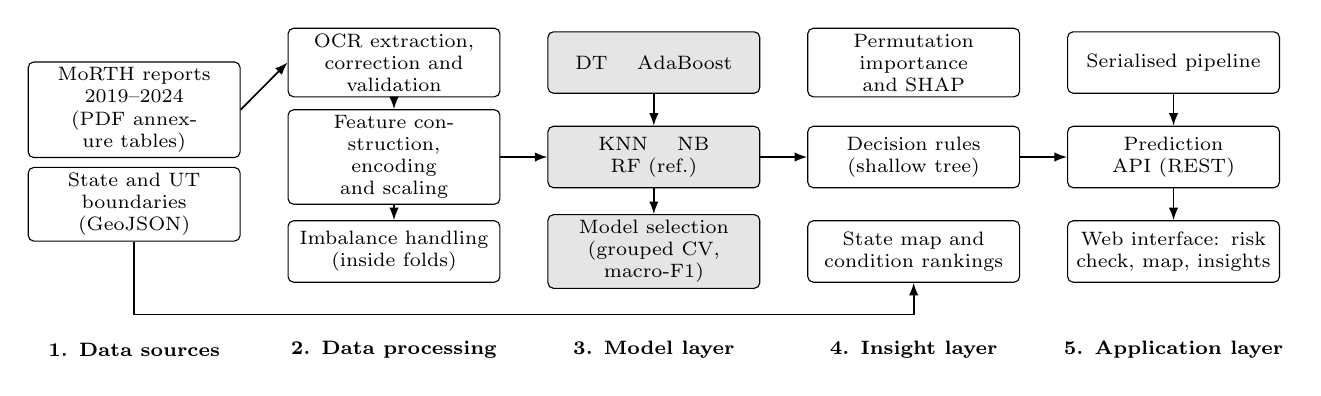
\begin{tikzpicture}[font=\scriptsize,
  box/.style={draw, rounded corners=2pt, align=center, text width=2.55cm, minimum height=0.78cm, inner sep=2pt},
  model/.style={box, fill=gray!20},
  arr/.style={-{Latex[length=1.6mm]}, semithick}]
% 1. data sources
\node[box] (s1) at (0,0.6) {MoRTH reports 2019--2024\\(PDF annexure tables)};
\node[box] (s2) at (0,-0.6) {State and UT boundaries\\(GeoJSON)};
% 2. data processing
\node[box] (p1) at (3.3,1.2) {OCR extraction,\\correction and validation};
\node[box] (p2) at (3.3,0) {Feature construction,\\encoding and scaling};
\node[box] (p3) at (3.3,-1.2) {Imbalance handling\\(inside folds)};
% 3. model layer
\node[model] (m1) at (6.6,1.2) {DT \quad AdaBoost};
\node[model] (m2) at (6.6,0) {KNN \quad NB \quad RF (ref.)};
\node[model] (m3) at (6.6,-1.2) {Model selection\\(grouped CV, macro-F1)};
% 4. insight layer
\node[box] (i1) at (9.9,1.2) {Permutation importance\\and SHAP};
\node[box] (i2) at (9.9,0) {Decision rules\\(shallow tree)};
\node[box] (i3) at (9.9,-1.2) {State map and\\condition rankings};
% 5. application layer
\node[box] (u1) at (13.2,1.2) {Serialised pipeline};
\node[box] (u2) at (13.2,0) {Prediction API (REST)};
\node[box] (u3) at (13.2,-1.2) {Web interface: risk\\check, map, insights};
% flows
\draw[arr] (s1.east) -- (p1.west);
\draw[arr] (p1) -- (p2);
\draw[arr] (p2) -- (p3);
\draw[arr] (p2.east) -- (m2.west);
\draw[arr] (m1) -- (m2);
\draw[arr] (m2) -- (m3);
\draw[arr] (m2.east) -- (i2.west);
\draw[arr] (i2.east) -- (u2.west);
\draw[arr] (u1) -- (u2);
\draw[arr] (u2) -- (u3);
\draw[arr] (s2.south) |- (9.9,-2.0) -- (i3.south);
% layer labels
\node at (0,-2.45) {\textbf{1. Data sources}};
\node at (3.3,-2.45) {\textbf{2. Data processing}};
\node at (6.6,-2.45) {\textbf{3. Model layer}};
\node at (9.9,-2.45) {\textbf{4. Insight layer}};
\node at (13.2,-2.45) {\textbf{5. Application layer}};
\end{tikzpicture}
\caption{Five-layer system architecture. The model layer (shaded) is evaluated under the leakage-safe protocol of Section~\ref{sec:method}.}
\label{fig:architecture}
\end{figure*}

% =====================================================================
\section{Implementation}
\label{sec:implementation}

The framework is implemented in Python~3.11 using pandas, scikit-learn \cite{pedregosa2011}, imbalanced-learn \cite{lemaitre2017}, SHAP \cite{lundberg2017} and scikit-posthocs, with Matplotlib for the figures. The prediction service is a Flask REST API with four endpoints (health check, valid options, prediction and map data); it validates every input, listens on the local interface only and accepts browser requests only from the front end. The front end is a single HTML page that uses Leaflet for the map.

One command runs the whole pipeline in six phases---prepare, train, evaluate, robustness, explain and insights---and regenerates every table and figure in this paper. The random seed is 42 for every estimator, resampler, shuffled split, permutation and sample.
% AUTHOR: add the public repository URL here if the code is released.

% =====================================================================
\section{Dataset Description}
\label{sec:dataset}

\subsection{Source}
The dataset is compiled from the annual MoRTH publication \emph{Road Accidents in India} \cite{morth2022,morthseries}, editions 2019 to 2024, prepared by the Ministry's Transport Research Wing from police records reported by the States and UTs. The reports publish State- and UT-wise tables in their annexures. Nine of these tables, each a different breakdown of the same accidents, are used (Table~\ref{tab:groups}).

\begin{table}[t]
\caption{Factor Groups and Role of Each Column}
\label{tab:groups}
\centering
\footnotesize
\begin{tabular}{@{}p{2.4cm}p{5.6cm}@{}}
\toprule
Group & Content \\
\midrule
\multicolumn{2}{@{}l}{\emph{Factor groups (source annexure)}} \\
Collision type (20) & Hit and run, head on, run off road, overturn, \ldots \\
Road environment (21) & Residential, institutional, market, open area \\
Road feature (22) & Straight, curved, bridge, culvert, pothole, steep grade, road works \\
Junction type (23) & T, Y, four-arm, staggered, roundabout \\
Traffic control (24) & Signal, police, stop sign, blinker, uncontrolled \\
Weather (25) & Clear, rain, fog, hail or sleet, others \\
Impacting vehicle (26) & Two-wheeler, car, truck, bus, pedestrian, \ldots \\
Traffic violation (35) & Over-speeding, drunken driving, wrong side, \ldots \\
Area type (39) & Rural, urban \\
\midrule
\multicolumn{2}{@{}l}{\emph{Used as features}} \\
Category & Factor group, factor value \\
Place & State (harmonised), region, State or UT \\
Other & Year, $\log(1+\text{accidents})$ \\
\midrule
\multicolumn{2}{@{}l}{\emph{Excluded (define the target)}} \\
Outcome counts & Killed, grievously injured, minor injured, total injured \\
Derived & Severity index, national severity \\
\bottomrule
\end{tabular}
\end{table}

\subsection{Compilation}
The annexures are printed tables inside PDF reports. Each annexure page was rendered at 400~dpi, the table grid lines were located with OpenCV, and each column was read with Tesseract optical character recognition. A misread value that broke a validation check was corrected only when the corrected value appears in the PDF's own text layer (2019--2023 editions) or a re-read of the single cell confirms it, and the check then passes; the 2024 corrections were verified against the printed page and the table's own totals. In total 79 cells were corrected, and every correction is logged with its page, State and column.

The result is a long-format panel of 11,752 rows and 17 columns, in which one row is one State or UT, one factor value and one year, with the numbers of accidents, persons killed, grievously injured and minor injured. Two units change during the period: Dadra \& Nagar Haveli and Daman \& Diu are reported separately in 2019 and merged afterwards, and Ladakh is reported with Jammu \& Kashmir in 2019--2020 and separately afterwards. A harmonised State attribute merges them into 35 units that are comparable across years.

\subsection{Validation}
Five checks were applied to the compiled panel:
\begin{enumerate}
\item Every column of every table sums to the All-India total printed in the report.
\item Grievously injured plus minor injured equals total injured in every row.
\item Collision type, road feature, weather, impacting vehicle, traffic violation and area type each reproduce the national numbers of accidents, persons killed and injured in every year.
\item For those groups, every State's sum equals its State total, with two exceptions that exist in MoRTH's printed 2020 tables: persons killed in Meghalaya in the impacting-vehicle table (6 more) and in Tamil Nadu in the road-feature table (1 more). These values are kept as printed.
\item The national totals match MoRTH's published figures (Table~\ref{tab:national}).
\end{enumerate}

\begin{table}[t]
\caption{National Totals in the Compiled Panel}
\label{tab:national}
\centering
\footnotesize
\begin{tabular}{@{}lrrr@{}}
\toprule
Year & Accidents & Persons killed & Severity index \\
\midrule
2019 & 449,002 & 151,113 & 33.66 \\
2020 & 366,138 & 131,714 & 35.97 \\
2021 & 412,432 & 153,972 & 37.33 \\
2022 & 461,312 & 168,491 & 36.52 \\
2023 & 480,583 & 172,890 & 35.98 \\
2024 & 487,707 & 177,175 & 36.33 \\
\bottomrule
\end{tabular}
\end{table}

\subsection{Target and Class Balance}
MoRTH defines the severity index as persons killed per 100 accidents. The target, the \emph{severity level} of a row, compares the row's severity index with the national severity index of the same year: Low if it is below 0.75 times the national value, High if it is above 1.25 times, and Medium otherwise. Rows with fewer than 10 accidents have no stable ratio and are excluded, which removes 2,420 rows and leaves 9,332 rows from 34 States and UTs for modelling. Table~\ref{tab:split} gives the class counts. The classes are only mildly imbalanced, and High is the largest class, not the rarest.

\begin{table}[t]
\caption{Rows and Classes in the Time Split}
\label{tab:split}
\centering
\footnotesize
\begin{tabular}{@{}llrrrr@{}}
\toprule
Split & Years & Rows & Low & Medium & High \\
\midrule
Train & 2019--2022 & 6,327 & 1,968 & 1,952 & 2,407 \\
Test & 2023--2024 & 3,005 & 883 & 913 & 1,209 \\
\midrule
All & 2019--2024 & 9,332 & 2,851 & 2,865 & 3,616 \\
\bottomrule
\end{tabular}
\end{table}

\subsection{Attribute Groups and Leakage Control}
Table~\ref{tab:groups} also lists the attributes used. The numbers of persons killed and injured, the severity index and the national severity define the target, so they are excluded from the features to prevent target leakage. The number of accidents is kept, on a logarithmic scale, because it describes exposure and does not by itself determine the ratio.

\subsection{Coverage Changes Between Years}
Three groups do not cover the same accidents in every year. Junction type and traffic control include an ``Others'' category covering all remaining accidents in 2019--2021 but report only junction accidents from 2022, when they cover between 20.1\% and 22.6\% of accidents. Road environment reports only residential, institutional and market areas in 2024, covering 41.2\% of accidents. Because every factor group is a separate breakdown of the same accidents, totals in this paper are always taken from one group (collision type) and never added across groups.

% =====================================================================
\section{Discussion: Outcomes}
\label{sec:discussion}

The study delivers the following outcomes, detailed in Section~\ref{sec:results}:
\begin{itemize}
\item a validated, reproducible benchmark of DT, AdaBoost, KNN and NB on State-level accident severity, reported with imbalance-aware metrics against a majority-class baseline (Table~\ref{tab:test});
\item evidence that the interpretable models are not statistically separable from one another on held-out States, and that only the reference RF differs from AdaBoost (Table~\ref{tab:friedman});
\item quantified effects of class weighting and oversampling, which are small and not consistently positive on these mildly imbalanced data;
\item evidence that performance does not transfer to States absent from training, and a leakage audit that quantifies two common pitfalls (Table~\ref{tab:robustness});
\item explanations that agree across methods that geography dominates, and a working web application for severity prediction and State-level mapping.
\end{itemize}

% =====================================================================
\section{Methodology}
\label{sec:method}

Fig.~\ref{fig:method} shows the end-to-end methodology.

\begin{figure}[t]
\centering
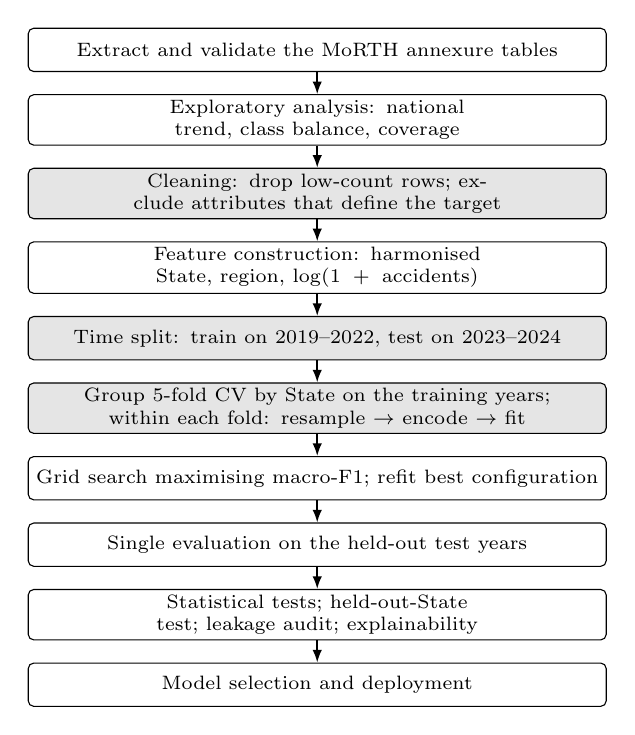
\begin{tikzpicture}[font=\scriptsize, node distance=0.28cm,
  stp/.style={draw, rounded corners=2pt, align=center, text width=7.2cm, minimum height=0.55cm, inner sep=2pt},
  risk/.style={stp, fill=gray!20},
  arr/.style={-{Latex[length=1.6mm]}, semithick}]
\node[stp] (a) {Extract and validate the MoRTH annexure tables};
\node[stp, below=of a] (b) {Exploratory analysis: national trend, class balance, coverage};
\node[risk, below=of b] (c) {Cleaning: drop low-count rows; exclude attributes that define the target};
\node[stp, below=of c] (d) {Feature construction: harmonised State, region, $\log(1+\text{accidents})$};
\node[risk, below=of d] (e) {Time split: train on 2019--2022, test on 2023--2024};
\node[risk, below=of e] (f) {Group 5-fold CV by State on the training years; within each fold: resample $\rightarrow$ encode $\rightarrow$ fit};
\node[stp, below=of f] (g) {Grid search maximising macro-F1; refit best configuration};
\node[stp, below=of g] (h) {Single evaluation on the held-out test years};
\node[stp, below=of h] (i) {Statistical tests; held-out-State test; leakage audit; explainability};
\node[stp, below=of i] (j) {Model selection and deployment};
\foreach \x/\y in {a/b,b/c,c/d,d/e,e/f,f/g,g/h,h/i,i/j} \draw[arr] (\x) -- (\y);
\end{tikzpicture}
\caption{Methodology. Shaded steps are where leakage is most often introduced in practice.}
\label{fig:method}
\end{figure}

\subsection{Preprocessing}
The compiled panel has no missing values in the modelling rows. For DT, AdaBoost, KNN and RF, the categorical attributes are one-hot encoded and the two numeric attributes are standardised. For NB, the categorical attributes and the year are ordinal-encoded for use with a categorical likelihood, and $\log(1+\text{accidents})$ is discretised into quartile bins. Some categories exist only in some years, and a split by State places unseen States in the validation fold; an unseen category is encoded as all zeros (one-hot) or as a reserved code that contributes only the smoothing term (NB).

\subsection{Feature Engineering}
Seven attributes are used: factor group, factor value, region, State or UT status, harmonised State, year and $\log(1+\text{accidents})$. The data contain no time of day, coordinates or driver attributes at this level of aggregation, so no temporal bands or weather merges are derived.

\subsection{Classification Algorithms}
\textbf{Decision Tree.} A CART tree \cite{breiman1984} recursively splits the data on the attribute that most reduces impurity. With Gini impurity at node $t$,
\begin{equation}
G(t) = 1 - \sum_{c=1}^{K} p_c(t)^2,
\end{equation}
where $p_c(t)$ is the proportion of class $c$ at $t$ and $K = 3$. Its root-to-leaf paths form human-readable rules.

\textbf{AdaBoost.} AdaBoost \cite{freund1997} builds an ensemble of shallow trees $h_m$ (depth 2 here), increasing the weights of misclassified samples after each round. In the multi-class SAMME form, the learner weight is
\begin{equation}
\alpha_m = \ln\frac{1-\varepsilon_m}{\varepsilon_m} + \ln(K-1),
\end{equation}
where $\varepsilon_m$ is the weighted error of $h_m$, and the final prediction is $\arg\max_c \sum_m \alpha_m \mathbf{1}[h_m(x) = c]$.

\textbf{k-Nearest Neighbours.} KNN \cite{cover1967} assigns a row the majority class among its $k$ nearest training rows, using Euclidean distance on the encoded attributes.

\textbf{Naive Bayes.} Categorical NB assumes attributes are conditionally independent given the class:
\begin{equation}
\hat{y} = \arg\max_c P(c) \prod_{j=1}^{d} P(x_j \mid c),
\end{equation}
with Laplace-smoothed likelihoods. It serves as a fast probabilistic baseline.

A Random Forest \cite{breiman2001} of 300 trees is also trained as a reference, so that the four models can be positioned against a strong ensemble.

\subsection{Imbalance Handling}
Three strategies are compared for each model:
\begin{enumerate}
\item \textbf{No handling}, as a baseline.
\item \textbf{Class weighting}, where each class $c$ with $n_c$ of $N$ training samples receives weight
\begin{equation}
w_c = \frac{N}{K\, n_c},
\end{equation}
so that errors on smaller classes cost more. DT and RF take the weights directly, AdaBoost receives them as sample weights, and NB uses a uniform class prior as its counterpart. KNN has no class-weight mechanism, so this combination is not run.
\item \textbf{Synthetic oversampling} with SMOTEN, the variant of SMOTE \cite{chawla2002} for categorical data, which uses the value difference metric \cite{stanfill1986}.
\end{enumerate}
Resampling is applied only to the training portion of each fold through an imbalanced-learn pipeline \cite{lemaitre2017}, so no synthetic sample is ever derived from validation or test rows. This gives 14 pipelines.

\subsection{Hyperparameter Tuning}
Hyperparameters are tuned by grid search on the training years with 5-fold cross-validation grouped by State, maximising macro-F1. Grouping keeps every State entirely in either the training or the validation part of a fold. Table~\ref{tab:grids} gives the search spaces. For each model, the strategy with the highest cross-validated macro-F1 is its \emph{selected configuration}; the test years play no part in this choice.

\begin{table}[t]
\caption{Hyperparameter Search Spaces}
\label{tab:grids}
\centering
\footnotesize
\begin{tabular}{@{}lp{6.4cm}@{}}
\toprule
Model & Grid \\
\midrule
DT & max depth $\in \{4, 6, 10, \text{none}\}$; min samples/leaf $\in \{1, 5, 20\}$ \\
AdaBoost & estimators $\in \{100, 300\}$; learning rate $\in \{0.1, 0.5, 1.0\}$ \\
KNN & $k \in \{5, 11, 21\}$; weights $\in \{\text{uniform}, \text{distance}\}$ \\
NB & smoothing $\alpha \in \{0.1, 0.5, 1.0\}$ \\
RF (ref.) & 300 trees; max depth $\in \{10, \text{none}\}$; min leaf $\in \{1, 5\}$ \\
\bottomrule
\end{tabular}
\end{table}

\subsection{Explainability}
Three methods are used. Permutation importance---the drop in macro-F1 when an attribute's values are shuffled, averaged over 10 repeats---is computed on the test set for the best interpretable model. A shallow tree (depth 4, at least 30 rows per leaf, balanced class weights) is trained for practitioners and its rules are extracted; splits whose two sides predict the same class are merged, and rules are ranked by weighted relative accuracy, that is, coverage multiplied by the excess of the rule's precision over the base rate of its class. SHAP values \cite{lundberg2017} explain the predictions of the best ensemble. Agreement between the top-ranked attributes across the three methods answers RQ3.

\subsection{Spatial Analysis}
The data identify the State but carry no coordinates, so density-based hotspot clustering is not possible. Instead, the severity index of each State is computed from summed counts for every year and drawn as a choropleth map, with the change from 2019 to 2024.

% =====================================================================
\section{Evaluation Design}
\label{sec:evaluation}

\subsection{Metrics}
With $TP_c$, $FP_c$ and $FN_c$ denoting true positives, false positives and false negatives for class $c$, per-class precision, recall and F1 are
\begin{equation}
P_c = \frac{TP_c}{TP_c + FP_c}, \qquad R_c = \frac{TP_c}{TP_c + FN_c},
\end{equation}
\begin{equation}
F1_c = \frac{2 P_c R_c}{P_c + R_c}.
\end{equation}
The primary metrics are macro-F1 and balanced accuracy, which weight every class equally:
\begin{equation}
\text{Macro-F1} = \frac{1}{K}\sum_{c=1}^{K} F1_c, \qquad \text{BA} = \frac{1}{K}\sum_{c=1}^{K} R_c,
\end{equation}
together with recall on each class, in particular High. Accuracy, one-vs-rest ROC-AUC and precision--recall AUC, both macro-averaged, are secondary metrics. Every pipeline is scored once on the test years, next to a baseline that always predicts the most common training class.

\subsection{Statistical Comparison}
Each model's selected configuration is re-evaluated on the training years with repeated grouped cross-validation: 5 folds grouped by State, repeated twice with different shuffles, with all models scored on the same 10 folds. The Friedman test on macro-F1, followed by the Nemenyi post-hoc test, determines whether differences in average rank are statistically significant \cite{demsar2006}.

\subsection{Generalisability Test}
A second dataset with a shared attribute set is not available at this level of aggregation. Generalisability is therefore tested within the panel in two ways: across space, by holding out whole States (the grouped cross-validation above); and across time, by scoring the model trained on 2019--2022 separately on 2023 and on 2024.

\subsection{Leakage Audit}
To demonstrate why the protocol matters, control experiments on the Decision Tree compare the leakage-safe setup with two pitfalls: a random row split that places rows of the same State in both training and test data, and the retention of an attribute that defines the target (the severity index, or the number of persons killed). Hyperparameters are held at their tuned values, so only the split or the feature set changes.

% =====================================================================
\section{Results}
\label{sec:results}

\subsection{Model Comparison and Baseline (RQ1)}
Table~\ref{tab:test} reports all 14 pipelines on the 3,005 test rows, and Fig.~\ref{fig:bars} shows macro-F1 and High-class recall. The baseline, which always predicts High, reaches an accuracy of 0.402 but a macro-F1 of 0.191 and a balanced accuracy of 0.333. Every pipeline is far above it, with macro-F1 from 0.687 to 0.778.

In their selected configurations, the four core models are close: KNN with SMOTEN has macro-F1 0.730, balanced accuracy 0.733 and High recall 0.781; AdaBoost without handling 0.717, 0.718 and 0.733; DT with SMOTEN 0.711, 0.716 and 0.728; and NB with class weighting 0.707, 0.709 and 0.746. The reference RF with class weighting is highest on all three (0.778, 0.781 and 0.792). The single highest High recall, 0.828, belongs to KNN without handling, which also has the highest macro-F1 among the four core models (0.744). Fig.~\ref{fig:confusion} shows that most errors involve the Medium class, whose recall (0.544 to 0.694) is the lowest of the three for every pipeline except AdaBoost with class weighting.

\textbf{Answer to RQ1.} On the test years KNN ranks first among the four core models and NB last, but the spread in macro-F1 between their selected configurations is 0.023 (0.730 against 0.707), and the reference RF is 0.048 above KNN.

\begin{table*}[t]
\caption{Test-Set Performance on the 2023--2024 Data ($n = 3{,}005$). ROC-AUC and PR-AUC Are One-vs-Rest, Macro-Averaged. Bold Marks the Best Pipeline in Each Column; $^\ast$ Marks Each Model's Selected Configuration (Highest Tuning Macro-F1); $^\dagger$ Reference Model Only.}
\label{tab:test}
\centering
\footnotesize
\setlength{\tabcolsep}{5pt}
\begin{tabular}{@{}llrrrrrrrr@{}}
\toprule
Model & Strategy & Accuracy & Bal.\ acc. & Macro-F1 & Recall Low & Recall Med. & Recall High & ROC-AUC & PR-AUC \\
\midrule
Majority baseline & Always High & 0.402 & 0.333 & 0.191 & 0.000 & 0.000 & 1.000 & 0.500 & 0.333 \\
\midrule
Decision Tree & None & 0.693 & 0.692 & 0.687 & 0.821 & 0.544 & 0.711 & 0.872 & 0.768 \\
Decision Tree & Class weights & 0.735 & 0.734 & 0.733 & 0.783 & 0.673 & 0.748 & 0.874 & 0.762 \\
Decision Tree$^\ast$ & SMOTEN & 0.716 & 0.716 & 0.711 & 0.822 & 0.597 & 0.728 & 0.858 & 0.738 \\
AdaBoost$^\ast$ & None & 0.719 & 0.718 & 0.717 & 0.776 & 0.645 & 0.733 & 0.868 & 0.762 \\
AdaBoost & Class weights & 0.714 & 0.720 & 0.716 & 0.796 & \textbf{0.694} & 0.668 & 0.867 & 0.752 \\
AdaBoost & SMOTEN & 0.720 & 0.720 & 0.719 & 0.777 & 0.660 & 0.723 & 0.869 & 0.752 \\
KNN & None & 0.753 & 0.746 & 0.744 & 0.844 & 0.567 & \textbf{0.828} & 0.886 & 0.792 \\
KNN$^\ast$ & SMOTEN & 0.737 & 0.733 & 0.730 & 0.830 & 0.588 & 0.781 & 0.883 & 0.785 \\
Naive Bayes & None & 0.716 & 0.710 & 0.707 & 0.802 & 0.551 & 0.778 & 0.875 & 0.770 \\
Naive Bayes$^\ast$ & Class weights & 0.712 & 0.709 & 0.707 & 0.800 & 0.582 & 0.746 & 0.875 & 0.771 \\
Naive Bayes & SMOTEN & 0.716 & 0.711 & 0.708 & 0.805 & 0.552 & 0.776 & 0.875 & 0.772 \\
\midrule
Random Forest$^\dagger$ & None & 0.747 & 0.745 & 0.742 & 0.828 & 0.627 & 0.779 & 0.898 & 0.811 \\
Random Forest$^{\dagger\ast}$ & Class weights & \textbf{0.781} & \textbf{0.781} & \textbf{0.778} & \textbf{0.866} & 0.686 & 0.792 & \textbf{0.920} & \textbf{0.848} \\
Random Forest$^\dagger$ & SMOTEN & 0.746 & 0.747 & 0.744 & 0.831 & 0.664 & 0.747 & 0.899 & 0.813 \\
\bottomrule
\end{tabular}
\end{table*}

\begin{figure*}[t]
\centering
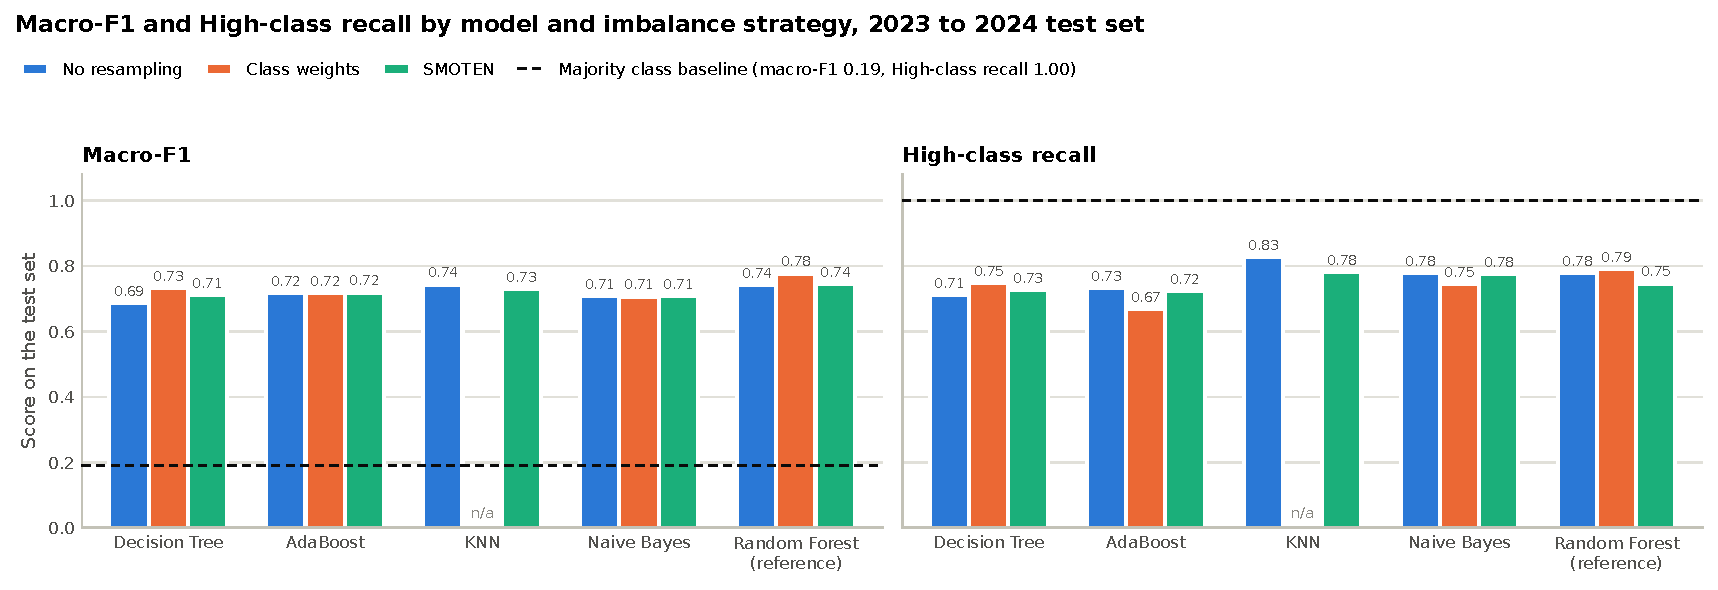
\includegraphics[width=0.92\textwidth]{fig08_macro_f1_high_recall}
\caption{Macro-F1 and High-class recall by model and imbalance strategy on the test years. The dashed line is the majority-class baseline.}
\label{fig:bars}
\end{figure*}

\begin{figure}[t]
\centering
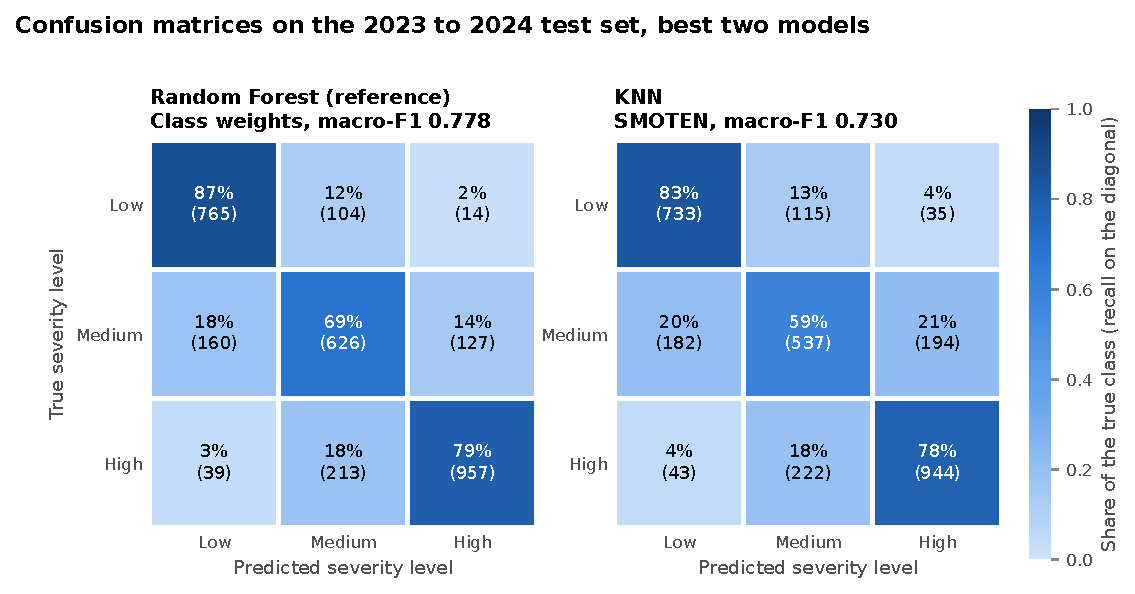
\includegraphics[width=\columnwidth]{fig07_confusion_matrices}
\caption{Confusion matrices on the test years for the two models with the highest test macro-F1 among the selected configurations.}
\label{fig:confusion}
\end{figure}

\subsection{Imbalance Strategies (RQ2)}
The effect of the strategies is small and not consistently positive. Relative to no handling, class weighting changes High recall by $+0.036$ for DT (0.711 to 0.748), $-0.065$ for AdaBoost (0.733 to 0.668), $-0.032$ for NB (0.778 to 0.746) and $+0.012$ for RF (0.779 to 0.792). SMOTEN changes it by $+0.017$ for DT, $-0.010$ for AdaBoost, $-0.047$ for KNN (0.828 to 0.781), $-0.002$ for NB and $-0.032$ for RF. Macro-F1 moves by at most 0.046, the gain of class weighting for DT (0.687 to 0.733); the next largest change is $+0.036$ for RF with class weighting, and all others are within 0.025.

Where the strategies do help, it is on the Medium class: class weighting raises Medium recall from 0.544 to 0.673 for DT, from 0.645 to 0.694 for AdaBoost, from 0.551 to 0.582 for NB and from 0.627 to 0.686 for RF.

\textbf{Answer to RQ2.} High recall improves only for DT ($+0.036$ with class weighting, $+0.017$ with SMOTEN) and for RF with class weighting ($+0.012$); it falls in the other six cases, by up to 0.065. The reason is in Table~\ref{tab:split}: High is the largest class (38.0\% of training rows), so rebalancing shifts predictions away from it and towards Medium.

\subsection{Statistical Comparison}
Table~\ref{tab:friedman} gives the repeated grouped cross-validation results for the selected configurations. The Friedman test rejects the hypothesis that the five models perform equally ($\chi^2(4) = 13.200$, $p = 0.010$). The Nemenyi critical difference at $\alpha = 0.05$ is 1.929 average ranks. Only one pair differs significantly: RF against AdaBoost ($p = 0.016$). KNN against AdaBoost is close to the threshold ($p = 0.056$). No pair among DT, AdaBoost, KNN and NB is significantly different, so the four core models cannot be ranked with confidence on unseen States.

\begin{table}[t]
\caption{Repeated Grouped Cross-Validation (5 Folds $\times$ 2 Repeats by State, 2019--2022) and Nemenyi $p$-Values}
\label{tab:friedman}
\centering
\footnotesize
\begin{tabular}{@{}lrrr@{}}
\toprule
Model (strategy) & Mean macro-F1 & SD & Avg.\ rank \\
\midrule
RF (class weights) & 0.454 & 0.084 & 2.0 \\
KNN (SMOTEN) & 0.447 & 0.087 & 2.3 \\
NB (class weights) & 0.425 & 0.087 & 2.9 \\
DT (SMOTEN) & 0.397 & 0.069 & 3.6 \\
AdaBoost (none) & 0.380 & 0.069 & 4.2 \\
\bottomrule
\end{tabular}

\vspace{4pt}
\begin{tabular}{@{}lrrrr@{}}
\toprule
 & AdaBoost & KNN & NB & RF \\
\midrule
DT & 0.915 & 0.351 & 0.860 & 0.157 \\
AdaBoost & & 0.056 & 0.351 & \textbf{0.016} \\
KNN & & & 0.915 & 0.993 \\
NB & & & & 0.708 \\
\bottomrule
\end{tabular}
\end{table}

\subsection{Robustness and Leakage (RQ4)}
Table~\ref{tab:robustness} reports the three control experiments on the Decision Tree.

\emph{Split design.} With whole States held out, the tree reaches a macro-F1 of 0.410. With a random stratified split of the same rows, which places each State on both sides, it reaches 0.750: an inflation of 0.340. The time split also contains every State on both sides, which explains why its score (0.711) is close to that of the random split; mixing the years as well adds a further 0.046.

\emph{Leakage.} Adding the severity index to the features lifts test macro-F1 from 0.711 to 0.981, because the target is defined from it. Adding the number of persons killed lifts it to 0.844, because together with the accident count it approximates the same ratio.

\emph{Drift.} The model trained on 2019--2022 scores 0.721 on 2023 and 0.701 on 2024, and High recall falls from 0.746 to 0.710.

\textbf{Answer to RQ4.} Performance does not transfer to unseen States: all five models score between 0.380 and 0.454 in grouped cross-validation (Table~\ref{tab:friedman}) against 0.707 to 0.778 on the time split (Table~\ref{tab:test}). Over time the decline is small, 0.019 in macro-F1 between the first and second test year.

\begin{table}[t]
\caption{Robustness Checks on the Decision Tree (SMOTEN). $\Delta$ Is the Change in Macro-F1 Against the Correct Setup Listed Before the Row in the Same Experiment. Cross-Validated Rows Report the Mean Over Five Folds.}
\label{tab:robustness}
\centering
\footnotesize
\setlength{\tabcolsep}{4pt}
\begin{tabular}{@{}p{2.75cm}rrrr@{}}
\toprule
Setup & Bal.\ acc. & Macro-F1 & Rec.\ High & $\Delta$ \\
\midrule
\multicolumn{5}{@{}l}{\emph{1. Split design}} \\
Grouped 5-fold by State & 0.416 & 0.410 & 0.465 & \\
Random stratified 5-fold & 0.751 & 0.750 & 0.813 & $+0.340$ \\
Time split & 0.716 & 0.711 & 0.728 & \\
Random rows, all years & 0.759 & 0.758 & 0.810 & $+0.046$ \\
\midrule
\multicolumn{5}{@{}l}{\emph{2. Leakage (time split)}} \\
Agreed features & 0.716 & 0.711 & 0.728 & \\
+ severity index & 0.983 & 0.981 & 0.972 & $+0.270$ \\
+ persons killed & 0.845 & 0.844 & 0.863 & $+0.132$ \\
\midrule
\multicolumn{5}{@{}l}{\emph{3. Drift (trained on 2019--2022)}} \\
Tested on 2023--2024 & 0.716 & 0.711 & 0.728 & \\
Tested on 2023 & 0.724 & 0.721 & 0.746 & $+0.009$ \\
Tested on 2024 & 0.708 & 0.701 & 0.710 & $-0.010$ \\
\bottomrule
\end{tabular}
\end{table}

\subsection{Explainability (RQ3)}
\emph{Permutation importance.} For the best interpretable model, NB with class weighting, shuffling the State lowers test macro-F1 by 0.307 (Fig.~\ref{fig:permutation}). The next attributes are the factor value (0.018), region (0.016), State or UT status (0.008), factor group (0.003) and the accident count (0.002). The year scores 0.000 by construction, since the test years are unseen categories for NB.

\emph{Decision rules.} The shallow tree has 15 leaves, which merge into 8 distinct rules, and reaches a test macro-F1 of 0.555. Table~\ref{tab:rules} lists the five most useful rules. All five are conditions on geography; the only other attribute that changes a prediction anywhere in the tree is the accident count, within Telangana. The first rule covers 4,352 of the 6,327 training rows and is correct for 0.537 of them, so it is a broad default, not a sharp finding.

\emph{SHAP.} For the best ensemble, RF with class weighting, the mean absolute SHAP value over the three classes, summed over each attribute's encoded columns, is 0.153 for State, 0.106 for region and 0.056 for State or UT status, ahead of the factor value (0.048), factor group (0.027), accident count (0.025) and year (0.016). Fig.~\ref{fig:shap} shows the direction: being in the South lowers the predicted probability of High, and being in the East or North raises it.

\textbf{Answer to RQ3.} The State is the most influential attribute under all three methods and for all three models examined (NB, DT and RF), followed by region. The crash condition has a real but much smaller influence: its permutation importance is 0.018 against 0.307 for the State.

\begin{table}[t]
\caption{The Five Most Useful Rules of the Shallow Decision Tree. Precision Is the Share of Covered Rows That Have the Predicted Level.}
\label{tab:rules}
\centering
\footnotesize
\begin{tabular}{@{}p{3.6cm}lrrr@{}}
\toprule
 & & Train & \multicolumn{2}{c}{Precision} \\
Rule & Level & rows & Train & Test \\
\midrule
Outside the South, except Jammu \& Kashmir and Ladakh, Madhya Pradesh and Goa & High & 4,352 & 0.537 & 0.570 \\
In the South, except Andhra Pradesh and Telangana & Low & 906 & 0.807 & 0.749 \\
In Jammu \& Kashmir and Ladakh & Low & 249 & 0.835 & 0.866 \\
In Madhya Pradesh & Low & 222 & 0.838 & 0.717 \\
In Andhra Pradesh & Medium & 219 & 0.813 & 0.743 \\
\bottomrule
\end{tabular}
\end{table}

\begin{figure}[t]
\centering
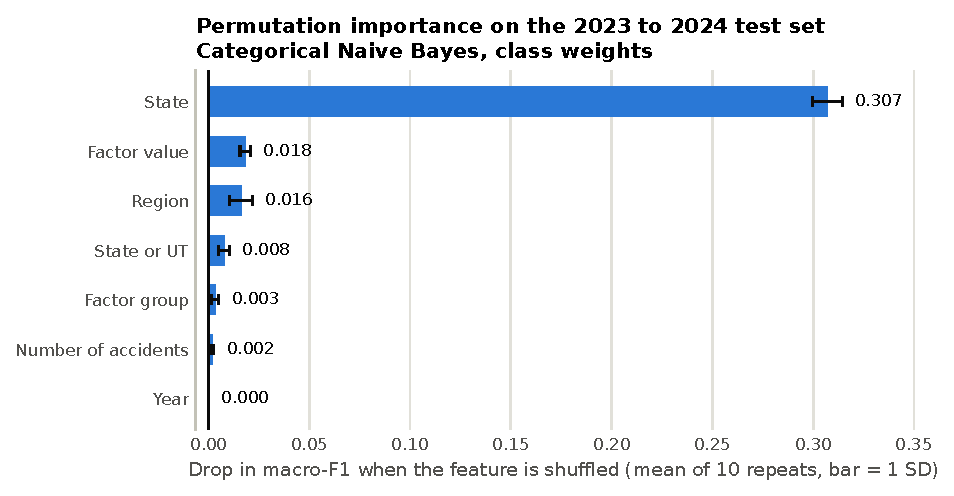
\includegraphics[width=\columnwidth]{fig09_permutation_importance}
\caption{Permutation importance on the test years for Categorical Naive Bayes with class weighting.}
\label{fig:permutation}
\end{figure}

\begin{figure}[t]
\centering
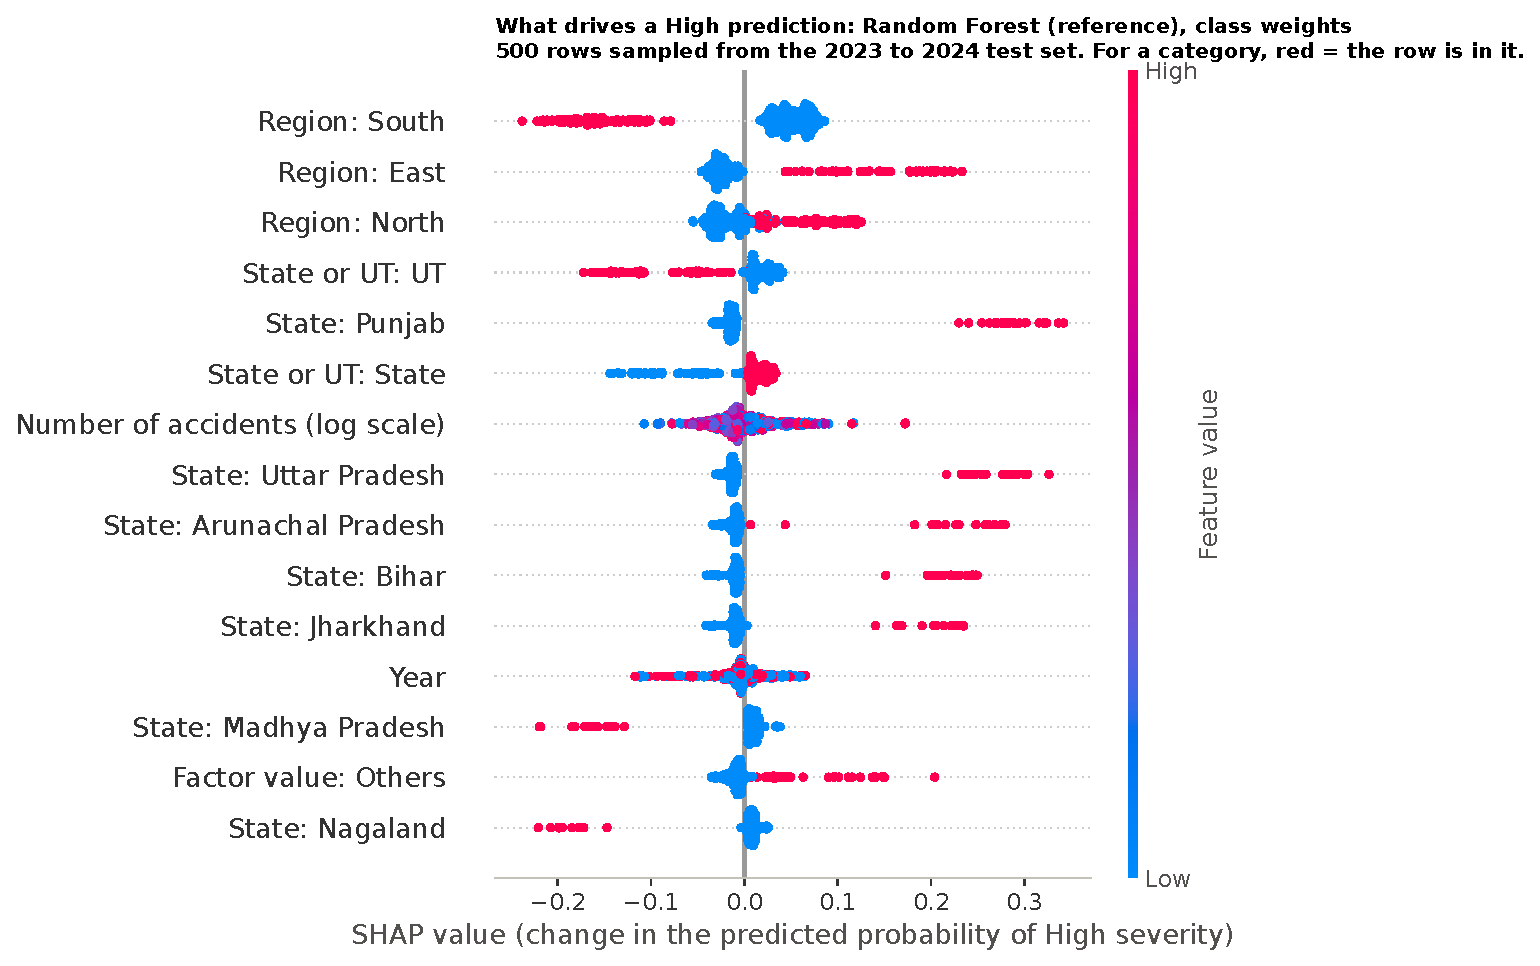
\includegraphics[width=\columnwidth]{fig10_shap_summary}
\caption{SHAP summary for the High class, Random Forest with class weighting, on 500 rows sampled from the test years.}
\label{fig:shap}
\end{figure}

\subsection{India Map and Insights}
The following findings come from the dataset alone, with severity always computed from summed counts.

\emph{National.} The severity index rose from 33.66 persons killed per 100 accidents in 2019 to 36.33 in 2024 (Table~\ref{tab:national}). Over the six years the panel records 2,657,174 accidents and 955,355 deaths, a severity of 35.95.

\emph{States.} Fig.~\ref{fig:map} maps severity in 2024 and its change since 2019. Among States with at least 500 accidents in both years, the highest values in 2024 are in Bihar (80.51), Jharkhand (79.18) and Punjab (78.49), and the lowest in Kerala (7.95) and Goa (10.66). The largest increases since 2019 are in Chhattisgarh ($+10.75$), Tamil Nadu ($+8.93$) and Bihar ($+8.51$), and the largest decrease is in West Bengal ($-5.42$).

\emph{Regions.} Severity over the six years ranges from 24.77 in the South and 28.25 in the Central region to 48.87 in the North and 59.76 in the East.

\emph{Conditions.} Table~\ref{tab:deadliest} ranks the deadliest conditions nationally. Hail or sleet (46.203), run-off-road (46.062), vehicle-overturn (45.821) and hit-and-run (45.330) accidents lead; hit and run is by far the largest of these, with 174,176 deaths. The association between severity level and factor value within a group is weak to moderate (Cram\'er's $V$ from 0.074 for road feature, not significant at $p = 0.477$, to 0.290 for area type), consistent with the small importance of the crash condition in the models.

\emph{State profile.} Karnataka, the State of the author's institution, has a severity of 28.49 over the six years against 35.95 nationally, and 28.77 against 36.33 in 2024, which ranks it 18th of the 25 States with at least 500 accidents.

\begin{figure*}[t]
\centering
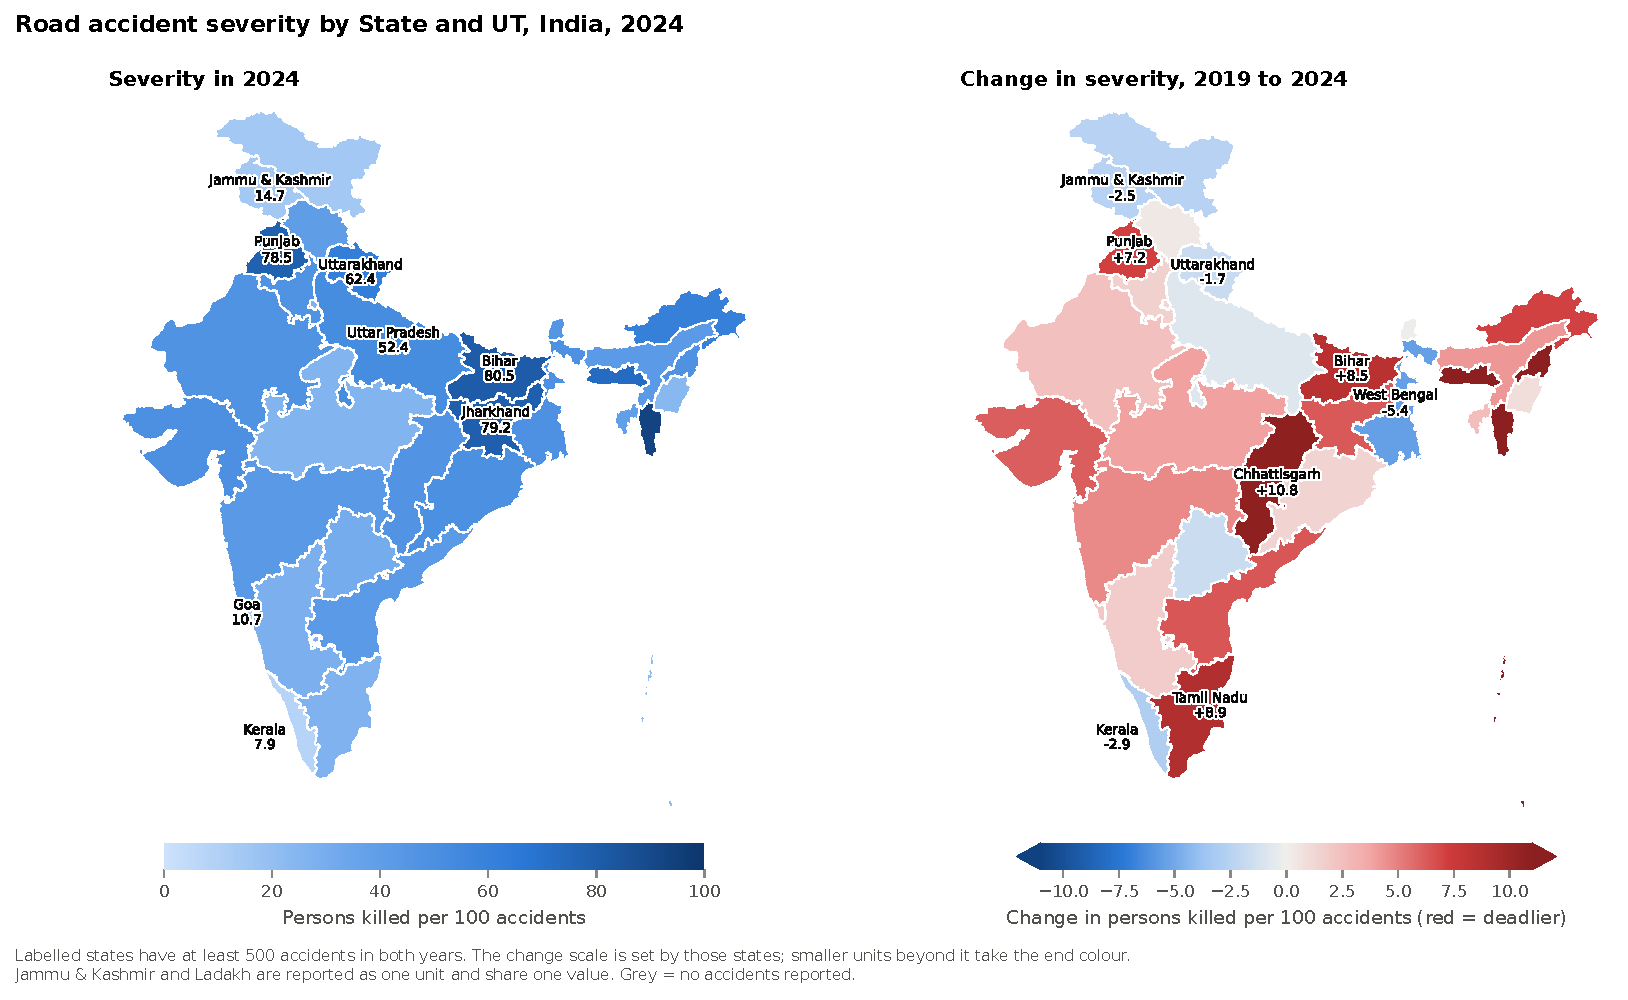
\includegraphics[width=0.86\textwidth]{fig11_state_severity_map}
\caption{Road accident severity (persons killed per 100 accidents) by State and UT in 2024, and the change from 2019.}
\label{fig:map}
\end{figure*}

\begin{table}[t]
\caption{The Ten Deadliest Conditions in India, 2019--2024 Combined (National Severity 35.95)}
\label{tab:deadliest}
\centering
\footnotesize
\setlength{\tabcolsep}{3.5pt}
\begin{tabular}{@{}p{2.5cm}p{1.2cm}rrr@{}}
\toprule
Condition & Group & Accidents & Deaths & Severity \\
\midrule
Hail/Sleet & Weather & 24,477 & 11,309 & 46.203 \\
Run off road & Collision & 117,942 & 54,326 & 46.062 \\
Vehicle overturn & Collision & 118,099 & 54,114 & 45.821 \\
Hit and run & Collision & 384,238 & 174,176 & 45.330 \\
Other non-motorised vehicle & Vehicle & 30,644 & 13,770 & 44.935 \\
Others & Vehicle & 146,831 & 65,761 & 44.787 \\
Fixed object & Collision & 90,890 & 40,497 & 44.556 \\
Use of mobile phone & Violation & 43,420 & 19,125 & 44.047 \\
Foggy \& Misty & Weather & 191,560 & 83,176 & 43.420 \\
Ongoing road works & Road feature & 59,241 & 25,710 & 43.399 \\
\bottomrule
\end{tabular}
\end{table}

\subsection{Web Application}
The application has three views. The risk check takes a State and a condition and returns the predicted level, the class probabilities, the three attributes with the largest SHAP contribution and the yearly severity record of that State and condition next to the national value. The map view shows the choropleth of Fig.~\ref{fig:map} for any year from 2019 to 2024. The insights view shows the rankings of Table~\ref{tab:deadliest}. The application serves the pipeline with the highest tuning macro-F1, which is the reference RF.

\subsection{Limitations}
\textbf{Aggregate data.} Every row is a yearly total for a State and a category, not a crash. The models classify categories of accidents in a State; they do not predict the outcome of an individual crash, and relationships seen in totals need not hold for individual crashes. The annexure tables are separate, so combinations of conditions (for example, rain on a curved road) are not available.

\textbf{Time split.} The time split tests on later years of States that were present in training. Its scores (macro-F1 0.707 to 0.778) therefore measure prediction for known States, and the grouped results (0.380 to 0.454) show that they do not hold for a State without history. The test period is two years, and the drift estimate rests on two points.

\textbf{Category changes.} Junction type, traffic control and road environment do not cover the same accidents in every year (Section~\ref{sec:dataset}), and two administrative units were merged or split during the period. Comparisons across years for these groups need care.

\textbf{Reporting and source quality.} The severity index is a ratio of reported counts, so it rises where minor accidents go unreported, and differences between States partly reflect reporting practice. The tables were extracted by OCR with 79 logged corrections, and two small inconsistencies in the printed 2020 tables are kept as published.

\textbf{Scope of the findings.} The classes are only mildly imbalanced, so the results on imbalance handling should not be generalised to data with a rare severe class. The Friedman and Nemenyi tests use 10 folds that share data and hyperparameters tuned on the same years, so their $p$-values are approximate. The SHAP analysis and the application use the reference RF, not one of the four core models.

% =====================================================================
\section{Conclusion}
\label{sec:conclusion}

This paper has presented and evaluated an interpretable, imbalance-aware and leakage-safe framework for road accident severity prediction on a validated panel of MoRTH statistics for 2019--2024. Under a common protocol, the four lightweight classifiers reach test macro-F1 between 0.707 and 0.730 in their selected configurations, against 0.191 for a majority-class baseline and 0.778 for the reference Random Forest; they are not statistically separable from one another on held-out States. Class weighting and SMOTEN change macro-F1 by at most 0.046 and raise High-class recall only for the Decision Tree and the Random Forest, because High is the largest class in these data.

The control experiments carry the main methodological message. A random row split inflates macro-F1 by 0.340 over a split by State, and leaking the severity index raises it from 0.711 to 0.981. All three explanation methods agree that the State carries most of the signal: the models describe where accidents are deadly far better than which conditions make them so, and they do not transfer to States without history.

These conclusions are bounded by the data: aggregate State-level counts, a time split that shares States between training and test years, and categories whose coverage changes across years. Future work will apply the framework to record-level crash data as they become available for Indian States, add features that describe States directly (such as road network, vehicle mix and emergency-care access) so that the State identifier is no longer needed, and tune decision thresholds for High-class recall.

\begin{thebibliography}{00}
\bibitem{who2023} World Health Organization, \emph{Global Status Report on Road Safety 2023}. Geneva, Switzerland: WHO, 2023.
\bibitem{morth2022} Ministry of Road Transport and Highways, Transport Research Wing, \emph{Road Accidents in India 2022}. New Delhi, India: Government of India, 2023.
\bibitem{behboudi2024} N. Behboudi, S. Moosavi, and R. Ramnath, ``Recent advances in traffic accident analysis and prediction: A comprehensive review of machine learning techniques,'' arXiv:2406.13968, 2024.
\bibitem{kapoor2023} S. Kapoor and A. Narayanan, ``Leakage and the reproducibility crisis in machine-learning-based science,'' \emph{Patterns}, vol. 4, no. 9, Art. no. 100804, 2023.
\bibitem{iranitalab2017} A. Iranitalab and A. Khattak, ``Comparison of four statistical and machine learning methods for crash severity prediction,'' \emph{Accident Analysis \& Prevention}, vol. 108, pp. 27--36, 2017.
\bibitem{almamlook2019} R. E. AlMamlook, K. M. Kwayu, M. R. Alkasisbeh, and A. A. Frefer, ``Comparison of machine learning algorithms for predicting traffic accident severity,'' in \emph{Proc. IEEE Jordan Int. Joint Conf. Electrical Engineering and Information Technology (JEEIT)}, Amman, Jordan, 2019, pp. 272--276.
\bibitem{shiran2021} G. Shiran, R. Imaninasab, and R. Khayamim, ``Crash severity analysis of highways based on multinomial logistic regression model, decision tree techniques, and artificial neural network: A modeling comparison,'' \emph{Sustainability}, vol. 13, no. 10, Art. no. 5670, 2021.
\bibitem{almistarehi2022} B. W. Al-Mistarehi, A. H. Alomari, R. Imam, and M. Mashaqba, ``Using machine learning models to forecast severity level of traffic crashes by R Studio and ArcGIS,'' \emph{Frontiers in Built Environment}, vol. 8, Art. no. 860805, 2022.
% AUTHOR: references mohamad2025, hoanglong2021, vanitha2023 and ethiopia2025 are incomplete in the earlier draft (no venue, volume or pages). Complete them before submission.
\bibitem{mohamad2025} I. Mohamad, S. Jomnonkwao, and V. Ratanavaraha, ``Machine learning predictive performance in road accident severity: A case study from Thailand,'' Elsevier, 2025.
\bibitem{hoanglong2021} Hoang Long, Ahmed, and Ma, ``A random forest approach to predicting traffic accident severity,'' 2021.
\bibitem{vanitha2023} Vanitha and Swedha, ``Prediction of road accidents using machine learning algorithms,'' 2023.
\bibitem{ethiopia2025} ``Predicting car accident severity in Northwest Ethiopia: A machine learning approach,'' 2025.
\bibitem{angarita2021} J. S. Angarita-Zapata, G. Maestre-Gongora, and J. F. Calder\'{\i}n, ``A bibliometric analysis and benchmark of machine learning and AutoML in crash severity prediction: The case study of three Colombian cities,'' \emph{Sensors}, vol. 21, no. 24, Art. no. 8401, 2021.
\bibitem{morthseries} Ministry of Road Transport and Highways, Transport Research Wing, \emph{Road Accidents in India}, annual editions 2019 to 2024. New Delhi, India: Government of India.
\bibitem{breiman1984} L. Breiman, J. Friedman, R. Olshen, and C. Stone, \emph{Classification and Regression Trees}. Belmont, CA, USA: Wadsworth, 1984.
\bibitem{freund1997} Y. Freund and R. E. Schapire, ``A decision-theoretic generalization of on-line learning and an application to boosting,'' \emph{J. Comput. Syst. Sci.}, vol. 55, no. 1, pp. 119--139, 1997.
\bibitem{cover1967} T. Cover and P. Hart, ``Nearest neighbor pattern classification,'' \emph{IEEE Trans. Inf. Theory}, vol. 13, no. 1, pp. 21--27, 1967.
\bibitem{breiman2001} L. Breiman, ``Random forests,'' \emph{Mach. Learn.}, vol. 45, no. 1, pp. 5--32, 2001.
\bibitem{chawla2002} N. V. Chawla, K. W. Bowyer, L. O. Hall, and W. P. Kegelmeyer, ``SMOTE: Synthetic minority over-sampling technique,'' \emph{J. Artif. Intell. Res.}, vol. 16, pp. 321--357, 2002.
\bibitem{stanfill1986} C. Stanfill and D. Waltz, ``Toward memory-based reasoning,'' \emph{Commun. ACM}, vol. 29, no. 12, pp. 1213--1228, 1986.
\bibitem{lemaitre2017} G. Lema\^{\i}tre, F. Nogueira, and C. K. Aridas, ``Imbalanced-learn: A Python toolbox to tackle the curse of imbalanced datasets in machine learning,'' \emph{J. Mach. Learn. Res.}, vol. 18, no. 17, pp. 1--5, 2017.
\bibitem{lundberg2017} S. M. Lundberg and S.-I. Lee, ``A unified approach to interpreting model predictions,'' in \emph{Advances in Neural Information Processing Systems 30}, 2017, pp. 4765--4774.
\bibitem{demsar2006} J. Dem\v{s}ar, ``Statistical comparisons of classifiers over multiple data sets,'' \emph{J. Mach. Learn. Res.}, vol. 7, pp. 1--30, 2006.
\bibitem{pedregosa2011} F. Pedregosa \emph{et al.}, ``Scikit-learn: Machine learning in Python,'' \emph{J. Mach. Learn. Res.}, vol. 12, pp. 2825--2830, 2011.
\end{thebibliography}

\end{document}
